\documentclass[14pt]{extarticle}
\usepackage[english,ukrainian]{babel}
\usepackage[utf8]{inputenc}
\usepackage{amsmath,amssymb}
\usepackage{parskip}
\usepackage{graphicx}
\usepackage{tcolorbox}
\tcbuselibrary{skins}
\usepackage[framemethod=tikz]{mdframed}
\usepackage{chngcntr}
\usepackage{enumitem}
\usepackage{hyperref}
\usepackage{float}
\usepackage{subfig}
\usepackage{esint}
\usepackage[top=2.5cm, left=3cm, right=3cm, bottom=4.0cm]{geometry}
\usepackage[table]{xcolor}
\usepackage{algorithm}
\usepackage{algpseudocode}
\usepackage{listings}
\usepackage{dsfont}
\usepackage{centernot}

\title{Самостійна робота з курсу ``Теорія міри''}
\author{Студента 3 курсу групи МП-31 Захарова Дмитра}
\date{\today}

\begin{document}

\maketitle

\section*{Завдання}
\textbf{Умова.} Нехай $(\mathbb{R},\mathcal{S}_1,\lambda_1)$ є простором з мірою,
\[
f_n = \begin{cases}
    \ln |n|, & x \in \left[-\frac{1}{n},\frac{1}{n}\right] \setminus \{0\} \\
    0, & x \in \left(\mathbb{R} \setminus\left[-\frac{1}{n},\frac{1}{n}\right]\right) \cup \{0\}
\end{cases}, \; x \in \mathbb{R}
\]
\begin{enumerate}
    \item Чи є послідовність $\{f_n\}_{n \in \mathbb{N}}$ збіжною майже скрізь відносно міри $\lambda_1$ на $\mathbb{R}$?
    \item Чи є послідовність $\{f_n\}_{n \in \mathbb{N}}$ збіжною за мірою $\lambda_1$ на $\mathbb{R}$?
\end{enumerate}

Якщо так, то знайти вiдповiднi границi. Вiдповiдi обґрунтувати.

\textbf{Розв'язок.} Спочатку спробуємо інтуїтивно інтерпретувати характер поведінки послідовності $\{f_n\}_{n \in \mathbb{N}}$. Отже, якщо спрямувати $n \to \infty$, то відрізок $[-\frac{1}{n},\frac{1}{n}]$ стає все вужчим, а значення $\ln|n|$ все більшим і асимптотично прямує до $+\infty$. Отже по своїй суті, $f_n$ мала б прямувати до функції Дірака $\delta(x)$, але на відміну від $\delta(x)$, $f_n(0)=0$. Тобто, дуже схоже, що для дуже великих $n \to \infty$ наша функція має стати ``еквівалентною'' $g \equiv 0$. 

Для ілюстративності, ми зобразили перші 100 функцій на рис \ref{fig:plot}. Дійсно можна побачити, що чим далі ми збльшуємо $n$, тим меньший шматок функції залишається на рівні $\ln n$. 

\begin{figure}[H]
    \centering
    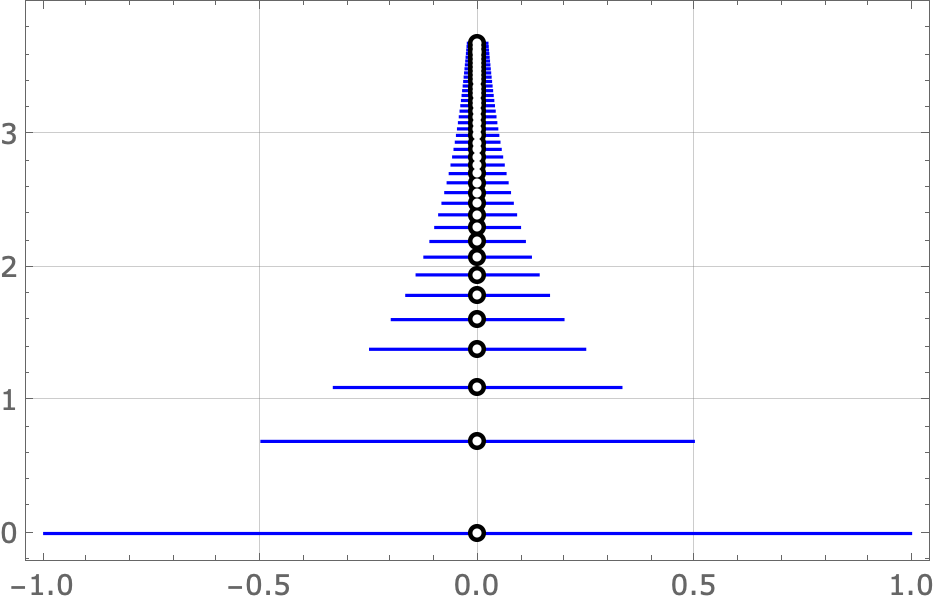
\includegraphics[width=0.7\textwidth]{images/hw_10.png}
    \caption{Перші 100 функцій $f_n$}
    \label{fig:plot}
\end{figure}

\textit{Пункт 1.} Нам потірбно знайти таку функцію $f$, що $f_n \to f\,(\text{mod}\,\lambda_1)$, тобто
\[
\exists N \subset \mathbb{R} \; \left(\lambda_1(N) = 0 \wedge \forall x \in \mathbb{R} \setminus N: \lim_{n \to \infty}f_n(x) = f(x)\right)
\]
В якості $N$ візьмемо $N = \{0\}$, тоді дійсно $\lambda_1(N)=0$. Тепер зафіксуємо будь-який $\omega \neq 0$ і порахуємо $\lim_{n \to \infty}f_n(\omega)$. Доведемо, що
\[
\forall \omega \neq 0: \lim_{n \to \infty}f_n(\omega) = 0
\]
\textbf{Ідея:} для достатньо великого $n$ відрізок $[-\frac{1}{n},\frac{1}{n}]$ перестане покривати $\omega$ і $f_n$ стане дорівнювати $0$.

\textbf{Доведення.} Перепишемо $f_n(\omega)$ в наступному вигляді:
\[
f_n(\omega) = \begin{cases}
    \ln|n|, & |\omega| \leq \frac{1}{n} \\
    0, & |\omega| > \frac{1}{n}
\end{cases} = \ln n \cdot \mathds{1}_{[-\frac{1}{n},+\frac{1}{n}]}(\omega)
\]
Отже звідси випливає, що при усіх $n \geq 1+\frac{1}{|\omega|}: f_n(\omega)=0$. Тому якщо з деякого номера отримуємо тотожньо нуль, то $\lim_{n \to \infty}f_n(\omega)=0$. 

\textbf{Наслідок.} В такому разі при $N = \{0\}$ та $f \equiv 0$, отримуємо:
\[
f_n \to 0 \, (\text{mod} \, \lambda_1)
\]

\textit{Пункт 2.} За означенням, збіжність послідовності $\{f_n\}_{n \in \mathbb{N}}$ означає:
\[
\exists f: f_n \xrightarrow[]{\lambda_1} f \iff \forall \varepsilon > 0: \lambda_1\left(\{x \in \mathbb{R}: |f_n(x)-f(x)| \geq \varepsilon\}\right) \xrightarrow[n \to \infty]{} 0
\]
В якості кандидата беремо $f \equiv 0$. Тоді треба довести (або спростити) наступну тезу:
\[
\forall \varepsilon > 0: \lambda_1(\{x \in \mathbb{R}: |f_n(x)| \geq \varepsilon) \xrightarrow[n \to \infty]{} 0
\]
Подивимось, який вигляд має $U^{(n)}_{\varepsilon} := \{x \in \mathbb{R}: |f_n(x)| \geq \varepsilon\}$. По-перше, $U^{(n)}_{\varepsilon} \subset [-\frac{1}{n},\frac{1}{n}] \setminus \{0\}$, оскільки на інших значеннях маємо $0$, що не перевищує $\varepsilon>0$. Більш того, на усіх точках з $[-\frac{1}{n},\frac{1}{n}] \setminus \{0\}$ значення однакове і дорівнює $\ln n$, причому має виконуватись $\ln n \geq \varepsilon$, або відповідно просто $n \geq e^{\varepsilon}$. Отже, по своїй суті, або ми беремо усю множину $[-\frac{1}{n},\frac{1}{n}] \setminus \{0\}$, якщо виконується $n \geq e^{\varepsilon}$, або перед нами пуста множина:
\[
U^{(n)}_{\varepsilon} = \begin{cases}
    \left[-\frac{1}{n},\frac{1}{n}\right] \setminus \{0\}, & n \geq e^{\varepsilon} \\
    \emptyset, & n < e^{\varepsilon}
\end{cases}
\]
Тому:
\[
\lambda_1(U^{(n)}_{\varepsilon}) = \begin{cases}
    \lambda_1([-\frac{1}{n},\frac{1}{n}] \setminus \{0\}), & n \geq e^{\varepsilon} \\
    0, & n < e^{\varepsilon}
\end{cases} \implies \lambda_1(U^{(n)}_{\varepsilon}) =\begin{cases}
    \frac{2}{n}, & n \geq e^{\varepsilon} \\
    0, & n < e^{\varepsilon}
\end{cases}
\]
Остаточно:
\[
\lambda_1(U^{(n)}_{\varepsilon}) = \frac{2}{n} \cdot \mathds{1}_{[e^{\varepsilon},+\infty)}(n)
\]
Таким чином, треба перевірити:
\[
\forall \varepsilon > 0: \lim_{n \to \infty} \left(\frac{2}{n} \cdot \mathds{1}_{[e^{\varepsilon},+\infty)}(n)\right) = 0
\]
Дійсно, якщо взяти доволі великі $n$ (а саме $n > e^{\varepsilon}$), то ми зможемо зробити одиницею вираз $\mathds{1}_{[e^{\varepsilon},+\infty)}$, а вираз $\frac{2}{n}$ буде прямувати до нуля при подальшому збільшені $n$.

\textbf{Відповідь.} В обох випадках збігається до $0$.

\end{document}

